
\documentclass[journal,12pt,twocolumn]
{IEEEtran}
\usepackage[none]{hyphenat}
\usepackage{graphicx}
\usepackage{listings}
\usepackage[english]{babel}
\usepackage{graphicx}
\usepackage{caption} 
\usepackage{amsmath}
\usepackage{hyperref}
\usepackage{booktabs}
\usepackage{array}

\providecommand{\norm}[1]{\left\lVert#1\right\rVert}
\providecommand{\abs}[1]{\left\vert#1\right\vert}
\let\vec\mathbf
\newcommand{\myvec}[1]{\ensuremath{\begin{pmatrix}#1\end{pmatrix}}}
\newcommand{\mydet}[1]{\ensuremath{\begin{vmatrix}#1\end{vmatrix}}}
\providecommand{\brak}[1]{\ensuremath{\left(#1\right)}}




\title{\textbf{\\Assignment on circles}}
\author{Sireesha Abbavaram - FWC22060}
\begin{document}
\maketitle


\section{Question}\vspace{2mm}
\textbf{\textit{Find the centre of the circle passing through the point (0,1) and touching the curve $y=x^2$ at the point (2,4).}}
\vspace{5mm}

\begin{figure}[h!]
\centering
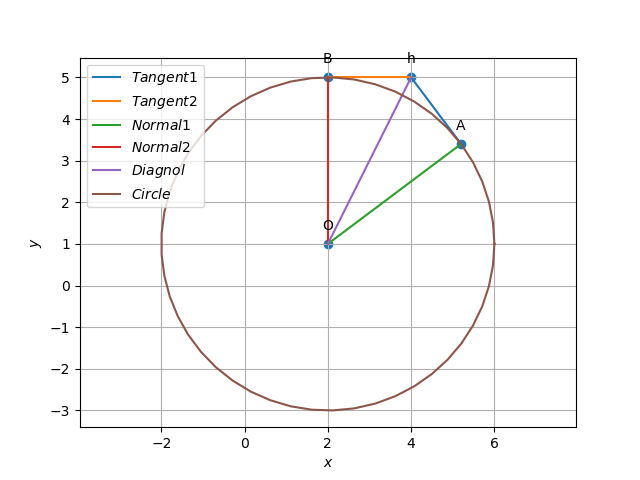
\includegraphics[scale=0.35]{circle.png}
\centering
\end{figure}



\section{Solution}
The equation of the circle is 
\begin{equation}
	x^T\vec{V}x + 2\vec{u}^Tx + f = 0
\end{equation}
Circle passes through $\myvec{0\\1}$ and  touches the curve $y=x^2$ at $\myvec{2\\4}$ 
Let $\vec{A}$=$\myvec{2\\4}$ and $\vec{B}$=$\myvec{0\\1} $
\begin{equation}
	\vec{A}\vec{A}^T + 2\vec{u}^T\vec{A} + f = 0
\end{equation}
\begin{equation}
	\norm{\vec{A}}^2 + 2\vec{A}^T \vec{u} + f = 0
\end{equation}
\begin{equation}
	\myvec{2\vec{A}^T & 1}\myvec{\vec{u} \\ f} = -\norm{A}^2 
\end{equation}
\begin{equation}
	\vec{B}\vec{B}^T + 2\vec{u}^T\vec{B} + f = 0
\end{equation}
\begin{equation}
	\norm{\vec{B}}^2 + 2\vec{B}^T\vec{u} + f = 0
\end{equation}
\begin{equation}
	\myvec{2\vec{B}^T & 1}\myvec{\vec{u} \\ f} = -\norm{\vec{B}}^2
\end{equation}
The equation of the tangent is
\begin{equation}
	\vec{m}^T (\vec{V}q + \vec{u}) = 0
\end{equation}
\begin{equation}
	\vec{m}^T\vec{A} +\vec{m}^T\vec{u} = 0
\end{equation}
\begin{equation}
	 \vec{m}^T\vec{u} = -\vec{m}^T\vec{A}
\end{equation}
\begin{center}
Where m is the directional vector of tangent found from the equation of tangent $\vec{n}^T(\vec{x}-\vec{q})=0$ i.e $4x-y=4$
\end{center}
\begin{center}
n is the normal vector of the curve $y=x^2$ given as $\vec{n}=\vec{V}\vec{q}+\vec{u}$
\end{center}
\begin{center}
The directional vector is given as $\vec{m}^T=omat*\vec{n}$ $\vec{m}=\myvec{-1 \\-4}$
\end{center}
from equations (4),(7) and (10),we can write as 
\begin{equation}
	\myvec{\vec{m}^T & 0 \\ 2\vec{A}^T & 1 \\ 2\vec{B}^T & 1}\myvec{\vec{u} \\ f} = \myvec{-\vec{m}^T\vec{A} \\ -\norm{\vec{A}}^2 \\ -\norm{\vec{B}}^2}
\end{equation}

\begin{center}
$\myvec{1&4&0&-18 \\4 & 8& 1 & -20 \\ 0 & 2 & 1 & -1 } \xrightarrow[]{R_1 \leftarrow -R1 }$\\
$\myvec{1&4&0&-18 \\1 & 2 & 1/4 & -5 \\ 0 & 2 & 1 & -1 } \xrightarrow[]{R_2 \leftarrow R2 / 4 } $\\
$\myvec{1&4&0&-18 \\0 & -2 & 1/4 & -13 \\ 0 & 2 & 1 & -1 } \xrightarrow[]{R_2 \leftarrow  R_2-R_1 }$\\
$\myvec{1&4&0&-18 \\0 & 1 & -1/8 & -13/2 \\ 0 & 2 & 1 & -1 } \xrightarrow[]{R_2 \leftarrow - 1/2R_2 }$\\
$\myvec{1&4&0&-18 \\0 & 1 & -1/8 & -13/2 \\ 0 & 1 & 1/2 & -1/2 } \xrightarrow[]{R_3 \leftarrow 1/2R_3 }$\\
$\myvec{1&4&0&-18 \\0 & 1 & -1/8 & -13/2 \\ 0 & 0 & 5/8 & 6 } \xrightarrow[]{R_3 \leftarrow R_3 -R_2}$\\
$\myvec{1&4&0&-18 \\0 & 1 & -1/8 & -13/2 \\ 0 & 0 & 1 & 48/5 } \xrightarrow[]{R_3 \leftarrow 8/5R_3}$\\
$\myvec{1&4&0&-18 \\0 & 1 & 0 & -53/10 \\ 0 & 0 & 1 & 48/5 } \xrightarrow[]{R_2 \leftarrow R_2+1/8R_3}$\\
$\myvec{1&0&0& 16/5 \\0 & 1 & 0 & -53/10 \\ 0 & 0 & 1 & 48/5 } \xrightarrow[]{R_1 \leftarrow R_1-4R_2}$\\

\end{center}
\begin{center}
By solving the above equations $\vec{u} =\myvec{16/5 \\ -53/10}$
The center is $\vec{C}$=-$\vec{u}$
therefore $\vec{C} = \myvec{-16/5 \\ 53/10}$
 and $f = 48/5$ 

\end{center}


\vspace{0.6cm}
Get the python code of the figures from
\begin{table}[h]
\large
\centering
\begin{tabular}{|l|}
\hline
https://github.com/Sireesha1602/sireesha/
\\blob/main/circleassignment\\
\hline
\end{tabular}

\end{table}


\end{document}
















